\chapter{SUMMARY AND FUTURE WORK}
\section{Summary}
This thesis presented the design, demonstration, and evaluation of a miniaturized and ruggedized single-ended laser-absorption-spectroscopy (SE-LAS) sensor for measuring gas temperature and $H_2O$ mole fraction in high-temperature combustion environments. The SE-LAS sensor presented here employs a single 6 $mm$ diameter lens, fiber-bundle, and custom body to provide high-fidelity measurements of gas properties while avoiding the use of windows and enabling convenient, alignment-free (after initial assembly) installation in compact locations. Most significantly, it was demonstrated that the SE-LAS sensor can repeatedly withstand direct exposure to high-temperature ($\approx 1000 \,K$) combustion gases for extended periods of time (at least 30 min) without compromising optical throughput or measurement quality. Using wavelength-modulation-spectroscopy techniques, the SE-LAS sensor demonstrated the ability to provide measurements of temperature and $H_2O$ mole fraction at a measurement bandwidth up to 25 $kHz$ and with a precision and accuracy that is comparable to or better than those of a conventional line-of-sight-based LAS sensor. Further, it was shown that the SE-LAS sensor presented here achieved an optical collection efficiency that is comparable (within 0.5$x$) to that of a previously developed SE-LAS sensor which employed an 18x larger-area lens.
In addition, a simple strategy for reducing the computational time required to perform scanned-WMS-$2f/1f$ spectral-fitting was presented. By storing previously calculated scanned-WMS-$2f/1f$ spectra in a look-up library, the best-fit spectra can be determined 100x faster and with an accuracy that is comparable to conventional non-linear least-squares fitting routines that have been used extensively \cite{Goldenstein:16}. This technique enabled the large dataset (240,000 spectra) acquired here to be processed in less than 7 hours instead of 28 days.

\section{Future Work}
\subsection{Field test in an exhaust aftertreatment system}
In Chapter 4, the compact single-ended LAS sensor was demonstrated in a laboratory-scale burner with great precision, accuracy and collection efficiency. In future work, this sensor will be applied to measure temperature and $H_2O$ in a Cummins exhaust aftertreatment system located in the Herrrick Laboratories. The modern diesel exhaust aftertreatment system includes Diesel Oxidation Catalyst (DOC), Diesel Particulate Filters (DPF) and Selective Catalytic Reduction (SCR) catalysts.The DOC and DPF are the first two devices in the aftertreatment system, where DOC oxidizes hydrocarbons, carbon monoxide and unburned fuel, and the DPF filters the remaining soot. SCR system is capable of converting $NO_x$ into water and nitrogen with the aid of urea injection and catalysts. The SCR has been extensively developed and analyzed by many researchers due to its great $NO_x$ reduction efficiency \cite{asif2015urea,southern1993demonstration,recsitouglu2015pollutant,GUAN2014395,doi:10.1177/0142331216656754,qi2003performance,saito2003development,muzio2002overview,gieshoff2000improved,sluder2005low,lei2013influence}. During the operation, the urea decomposes constantly into ammonia ($NH_3$) as the reactant. The reaction temperature will be a critical factor in the performance evaluation of the SCR system due to the high thermal sensitivity of the urea decomposition rate and chemical kinetics. SE-LAS sensors have advantages of taking a non-intrusive and rapid measurement of gas temperature and $H_2O$.

 \begin{figure}[ht]
    \centering       
    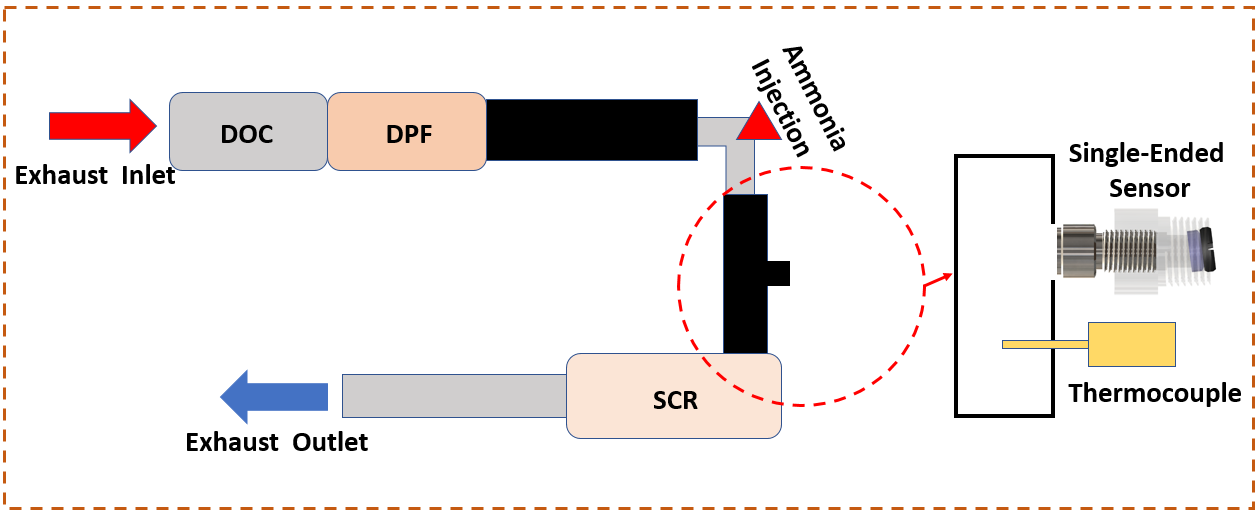
\includegraphics[width=0.8\textwidth]{fig/ch5_fig1.PNG}
        \caption{Schematic of proposed field test of the single-ended temperature and $H_2O$ sensor in the Cummins exhaust aftertreatment system.}
    \label{fig:ch5_1}
\end{figure}

Fig. 5.1 illustrates a schematic of the planned field test with the single-ended sensor in a Cummins exhaust aftertreatment system. The sensor is located upstream of SCR to measure the temperature and $H_2O$ mole fraction with sub-millisecond response time. Furthermore, this sensor can be deployed in more locations (such as downstream of SCR) with/without the urea injection. Several challenges may need to be overcome including: 1) the corrosion on the lens by direct exposure to high-temperature exhaust gas; 2) condensation of $H_2O$ on the lens which could decrease the collection efficiency. 
 
